%% This is file `elsarticle-template-1-num.tex',

\documentclass[preprint,12pt]{elsarticle}

%% The graphicx package provides the includegraphics command.
\usepackage{graphicx}
%% The amssymb package provides various useful mathematical symbols
\usepackage{amssymb}
%% The amsthm package provides extended theorem environments
%% \usepackage{amsthm}
\usepackage{lineno}
\usepackage{color}
\usepackage{sectsty}
\subsubsectionfont{\normalfont}
\subsectionfont{\normalfont}
\usepackage{multirow}
\usepackage{subfiles}


\journal{Journal Name}

\begin{document}

\begin{frontmatter}

%% Title, authors and addresses

\title{\texttt{UQpy} - Uncertainty Quantification with Python}
\author{Dimitris G. Giovanis, M. D. Shields}

\address{Johns Hopkins University, USA}

\end{frontmatter}

%%
%% Start line numbering here if you want
%%
\linenumbers
\section{Installing \texttt{UQpy}}

\underline{Prerequisites:}
You have at least one Python interpreter 3.6+ properly installed on your computer. In order to get the latest experimental version of  \texttt{UQpy} the code can be installed from Github directly as follows:

\begin{itemize}
\item[ ]  \texttt{\$git clone https://github.com/SURGroup/UQpy.git}
\item[ ] \texttt{\$cd UQpy/}
\item[ ] \texttt{\$pip install -r  requirements.txt}.
\item[ ]  \texttt{\$python setup.py install}.
\end{itemize}

\noindent
The last command might need \textbf{sudo} prefix, depending on your python setup. 

%% main text
\section{Overview}
\label{S:overview}
\noindent
\texttt{UQpy} (Uncertainty Quantification (UQ) using python) is a software toolbox containing a collection of modules  written in Python that provide standardized solutions for many UQ problems that occur in physical model. Connection between UQpy and the user-defined computational model is made with text-based and bash shell script(s) provided by the user. Execution of \texttt{UQpy} results in realizations of the parametric space of interest using advanced techniques, as well as evaluations the corresponding model responses. \texttt{UQpy} is entirely code-agnostic and gives users a fully functional tool for performing UQ with nearly any computational analysis code. \texttt{UQpy} performs submission, execution, monitoring and post-process analysis, specifically tailored to  the analysis tool and the available platform and thus, it is amenable to performing adaptive UQ methods. \texttt{UQpy} is written in the Python 3 programming language.

\subsection{Compiled version of \texttt{UQpy}}

\noindent
{\color{red} We need to address the Windows version}

\subsection{Interpreted version of \texttt{UQpy}}

\noindent
The interpreted version of \texttt{UQpy} requires a Python shell supporting Python 3.6+ as well as several common Python libraries as well.  After downloading and installing \texttt{UQpy}, the following \texttt{UQpy}-specific files are required and must be co-located in the subdirectory lib/\textbf{UQpy}, which is in the same directory as {\color{blue}UQpy\_cmd.py}:

\begin{itemize}
\item[$\cdot$] {\color{blue}UQpyModules.py} - Contains various functions.
\item[$\cdot$] {\color{blue}SampleMethods.py} - Contains the available sampling methods used for exploring the parameter space.
\item[$\cdot$] {\color{blue}ReadInputFile.py} -  Reads the necessary UQ Parameter data file  in case of running \texttt{UQpy}  via command line, and converts it to  python variables. 
\item[$\cdot$] {\color{blue}PDFs.py} - Contains the percent point functions of all the supported distributions; any new distribution can be added here. 
\end{itemize}

\section{Using UQpy- Required files}

\noindent
\texttt{UQpy} may be run using either an Integrated Development Environment (IDE) used in computer programming, specifically for the Python language or via the command line. The interpreted version of \texttt{UQpy}, has been tested to run in IDE PyCharm 2017.3.3.

In order to use  \texttt{UQpy} for evaluating the response of any computational model for a number of parameter realizations,  \texttt{UQpy}  requires three \textbf{executable}\footnote{\$\texttt{chmod +x }{\color{red}name1*.sh} } bash shell scripts: 

\begin{itemize}
\item {\color{red}name1*.sh} for linking the analysis software to \texttt{UQpy} 

\item {\color{red}name2*.sh} for converting the the file containing the parameter values (text-based file) into appropriate input file for the analysis code  

\item {\color{red}name3*.sh} converting the result of the software analysis into an appropriate  (text-based) file to be read from \texttt{UQpy}. This is necessary  in case of running adaptive UQ methods and/or post-processing of the results. 
\end{itemize}

\noindent
The names of these files are user defined. Additional to these files, if the user wants to  generate the realizations of the random parameters according to one of the  available sampling methods  provided in \texttt{UQpy}, it is necessary to provide an text-based file under the name  ({\color{magenta}UQpy\_params.txt}), which will enclose all the probabilistic information required for running the selected sampling method. T

The aforementioned files are directly specified by the user and may be in any directory.


\section{UQpy Usage}

\noindent
\texttt{UQpy} is user friendly since it only requires the user to have basic knowledge in writing bash shell scripts.

\subsection{Using the \texttt{UQpy}  Command Line Mode}

\noindent
\texttt{UQpy} can be executed directly through the command line. It is provided as an option to the user who doesn't have sufficient familiarity and experience with python. Command line execution is advantageous when analyses need to be performed on a high-performance computing systems without direct graphics capability. In order to  execute the interpreted version \texttt{UQpy} from the command line the user needs to  change to the \texttt{UQpy} directory and then type in terminal :

\vspace{4mm}
\noindent
{\scriptsize \texttt{\$python UQpy\_cmd.py --dir pathToModel --model name1*.sh --input name2*.sh --output name3*.sh}}


\vspace{4mm}
\noindent
Where

\begin{itemize}
 \item  {\color{blue} UQpy\_cmd.py} is the python script that actually runs \texttt{UQpy}  via command line and needs to be located in the directory \textbf{UQpy}.
 
 \item \texttt{--dir} is the absolute path to the folder which contains the necessary files  {\{\color{red}name1*.sh} , {\color{red}name2*.sh} , {\color{red}name3*.sh} and {\color{magenta}UQpy\_params.txt}\}.
 
 \item \texttt{--model} points to the {\color{red}name1*.sh} bash script
 
  \item \texttt{--input} points to the {\color{red}name2*.sh} bash script
  
   \item \texttt{--output} points to the {\color{red}name3*.sh} bash script
 
 \end{itemize}


\noindent
In order for \texttt{UQpy}  to run from command line  the file  {\color{magenta}UQpy\_params.txt} is necessary to be located inside \texttt{--dir} otherwise, the execution will return an error. However the user may skip the entries \{\texttt{--input, --output, --model}\}  if  \texttt{UQpy}  is utilized only for generating realizations of the random parameter and not for model evaluations.  Another optional entry for the user is \texttt{--CPUs} which sets the number of processors used for the evaluation of the model, in case of parallel processing.   The user can see all the available options (Fig. \ref{UQpy_help}) by typing in terminal

\vspace{4mm}
{\centering
	{\small \texttt{\$python UQpy\_cmd.py --help}}\par}
\vspace{4mm}


\noindent
which results in:

\begin{figure}[!ht]
	\centering	{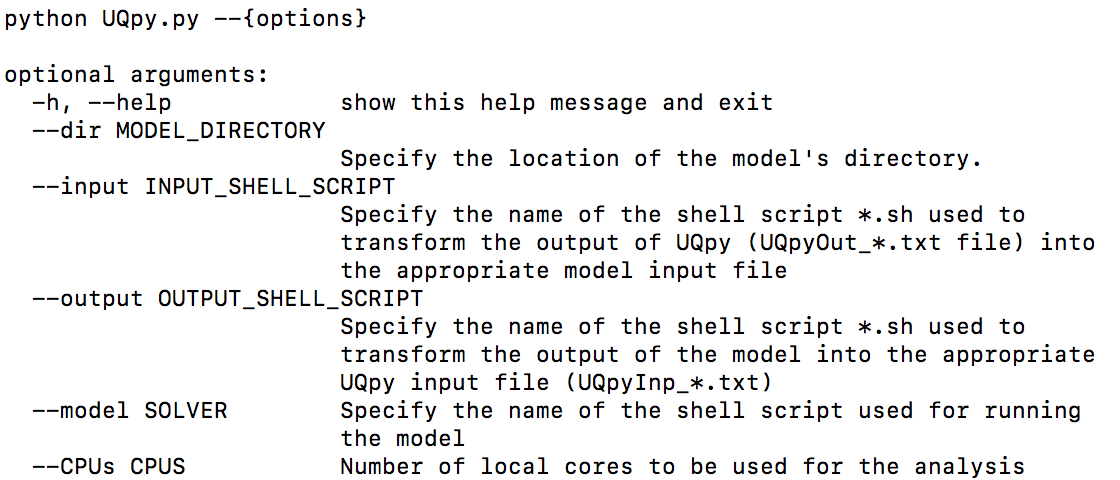
\includegraphics[scale=0.7]{UQpy_help}}
	\caption{}
	\label{UQpy_help}
\end{figure}


\subsection{Using the \texttt{UQpy}  IDE Mode}
\label{sec:IDE_Mode}

\noindent
After installation, \texttt{UQpy} is build in the local Python’s standard library and thus, it runs from any Integrated Development Environment (PyCharm, Atom, Eclipse, e.t.c) which provides code analysis and debugging. In order to use \texttt{UQpy} libraries in a project the user needs to import the specific module to its workspace. This can be done by writing in a python script

\vspace{4mm}
{\centering
 \texttt{{\color{blue} from} \texttt{UQpy} {\color{blue} import} * }\par}
\vspace{4mm}

\noindent
which will load all modules of \texttt{UQpy}. If a specific class from the sample methods  (e.g Monte Carlo simulation) is required then the user can selectively load it to the project by typing 
\vspace{4mm}

{\centering
 \texttt{{\color{blue} from} \texttt{UQpy.SampleMethods} {\color{blue} import} MCS }\par}

\vspace{4mm}
\noindent
This functionality of \texttt{UQpy} enables the independent usage of its  modules, which makes \texttt{UQpy} a powerful tool for UQ analysis and communication between python and various computational codes of different nature.  In order to generate 100 realizations of two random parameters using MCS  the user needs to type:
\vspace{4mm}

{\centering
	\texttt{{\color{blue} from} \texttt{UQpy.SampleMethods} {\color{blue} import} MCS }\\
	\texttt{x = MCS(dimension=2, pdf\_type=['Uniform', 'Uniform'])\\
	pdf\_params=[[0, 1], [0, 1] ], nsamples=100)}\par}

\vspace{4mm}
\noindent
This will create the object \texttt{x} with is properties:

\begin{itemize}
	\item[1.] \texttt{pdf\_type}: type of distribution for each parameter
	\item[2.] \texttt{pdf\_params}: distribution parameters
	\item[3.] \texttt{nsamples}: number of samples to be generated
	\item[4.] \texttt{dimension}: number of random parameters
	\item[5.] \texttt{samples}: generated samples in the parameter space
	\item[6.] \texttt{samplesU01}: generated samples in the Uniform space, U[0, $1]^{\mbox{\texttt{dimension}}}$
	\end{itemize}



\section{\texttt{UQpy} workflow}


\section{Templates for the required  Files}

\noindent
The interaction between \texttt{UQpy}  and any external solver is made  with text-based files which are simple to process and easy to work with in python.  

\subsection{Probabilistic Parameter File}

\noindent
The file that keeps the probabilistic properties of the parameters should always be under the name:

\vspace{4mm}
{\centering
{\color{magenta}UQpy\_params.txt}\par}

\vspace{4mm}
\noindent
Creating {\color{magenta}UQpy\_params.txt} is simple and straightforward; Each property that is required for the selected sampling method, is defined in a line  that starts  with a hash-tag (\#),  followed by a key-word and/or key-phrase (case sensitive) describing the property\footnote{The order that the properties are declared in {\color{magenta}UQpy\_params.txt} is not important .}. The file ends with the key-word \texttt{\#end}. Under that line, the specific attributes of the property are defined, according to the \texttt{UQpy} available options. Thus, different sampling methods require different parameter file . 

\subsubsection{Required properties for various sampling methods}

The properties that need to be specified by the user inside the parameter file in order to run different sampling methods, for exploring the parameter space. A summary of these properties  is given next:  

\begin{center}
	\begin{tabular}{ |l|c|c| } 
		\hline
		\multicolumn{3}{|c|}{\textbf{Monte Carlo simulation}} \\
		\hline
		\textbf{Property} & \textbf{Mandatory} & \textbf{Optional} \\
		\hline
		 \texttt{\#method}& $\star$ &   \\ 
		\hline
		\texttt{\#number of samples}& $\star$ &   \\ 
		\hline
		\texttt{\#number of parameters}& $\star$  &   \\ 
		\hline
		\texttt{\#distribution type}& $\star$ &   \\ 
		\hline
		\texttt{\#distribution parameters} & $\star$ &   \\ 
		\hline
		\texttt{\#names of parameters}& & $\star$   \\ 
		\hline
		\texttt{\#SROM}&  & \textbf{True} or \textbf{False}  \\ 
		\hline
	\end{tabular}
\end{center}

\begin{center}
	\begin{tabular}{ |l|c|c| } 
				\hline
		\multicolumn{3}{|c|}{\textbf{Latin hypercube simulation}} \\
		\hline
		\textbf{Property} & \textbf{Mandatory} & \textbf{Optional} \\
		\hline
		\texttt{\#method}& $\star$ &   \\ 
		\hline
		\texttt{\#number of samples}& $\star$ &   \\ 
		\hline
		\texttt{\#number of parameters}&  $\star$  &   \\ 
		\hline
		\texttt{\#distribution type}& $\star$ &   \\ 
		\hline
		\texttt{\#distribution parameters} & $\star$ &   \\ 
		\hline
		\texttt{\#names of parameters}& & $\star$   \\ 
		\hline
		\texttt{\#criterion}& & $\star$   \\ 
		\hline
		\texttt{\#distance}& & $\star$   \\ 
		\hline
		\texttt{\#metric}& & $\star$   \\ 
		\hline
				\texttt{\#SROM}&  & \textbf{True} or \textbf{False}    \\ 
		\hline
	\end{tabular}
\end{center}

\begin{center}
	\begin{tabular}{ |l|c|c| } 
		\hline
		\multicolumn{3}{|c|}{\textbf{Stratified sampling}} \\
		\hline
		\textbf{Property} & \textbf{Mandatory} & \textbf{Optional} \\
		\hline
		\texttt{\#method}& $\star$ &   \\ 
		\hline
		\texttt{\#distribution type}& $\star$ &   \\ 
		\hline
		\texttt{\#number of parameters}& &$\star$    \\ 
		\hline
		\texttt{\#distribution parameters} & $\star$ &   \\ 
		\hline
		\texttt{\#design}& $\star$ &    \\ 
		\hline
		\texttt{\#names of parameters}& & $\star$   \\ 
		\hline
				\texttt{\#SROM}&  & \textbf{True} or \textbf{False}    \\ 
		\hline
	\end{tabular}
\end{center}

\begin{center}
	\begin{tabular}{ |l|c|c| } 
		\hline
		\multicolumn{3}{|c|}{\textbf{Partially Stratified sampling}} \\
		\hline
		\textbf{Property} & \textbf{Mandatory} & \textbf{Optional} \\
		\hline
		\texttt{\#method}& $\star$ &   \\ 
		\hline
		\texttt{\#distribution type}& $\star$ &   \\ 
		\hline
		\texttt{\#distribution parameters} & $\star$ &   \\ 
		\hline
		\texttt{\#number of parameters}& &$\star$    \\ 
		\hline
		\texttt{\#design}& $\star$  &  \\ 
		\hline
		\texttt{\#strata}& $\star$ &   \\ 
		\hline
		\texttt{\#names of parameters}& & $\star$   \\ 
		\hline
				\texttt{\#SROM}&  & \textbf{True} or \textbf{False}    \\ 
		\hline
	\end{tabular}
\end{center}




\begin{center}
	\begin{tabular}{ |l|c|c| } 
		\hline
		\multicolumn{3}{|c|}{\textbf{Stochastic reduced order model}} \\
		\hline
		\textbf{Property} & \textbf{Mandatory} & \textbf{Optional} \\
		\hline
		\multicolumn{3}{|c|}{If \texttt{\#SROM} property is \textbf{True}} \\
		\hline
		\texttt{\#moments}& $\star$ &   \\ 
		\hline
		\texttt{\#error function weights} & $\star$ &   \\ 
		\hline
		\texttt{\#properties to match}&  &  $\star$  \\ 
		\hline
		\texttt{\#sample weights}& & $\star$   \\ 
		\hline
	\end{tabular}
\end{center}


\subsubsection{Examples of parameter files}


\noindent
 Special instruction on how to create the parameter file that will enclose the required properties of the selected sampling method are the following :
 
 \begin{itemize}
 	 	\item  A complete parameter file for  e.g. Monte Carlo simulation can defined like Fig.\ref{template_mcs}(a).
 	
 	\item  If all random parameters follow the same distribution type with the same distribution parameters then a parameter file  can defined like Fig.\ref{template_mcs}(b) where the distribution type and parameters need to be defined once. In this case existence of the property  "number of random parameters" is mandatory.
 	
 	 \item  For the case the number of distribution type is equal to the number of distribution parameters (Fig.\ref{template_mcs}(c))  then, definition of property "number of parameters" is optional .
 	\end{itemize}


\begin{figure}[!ht]
	\centering	{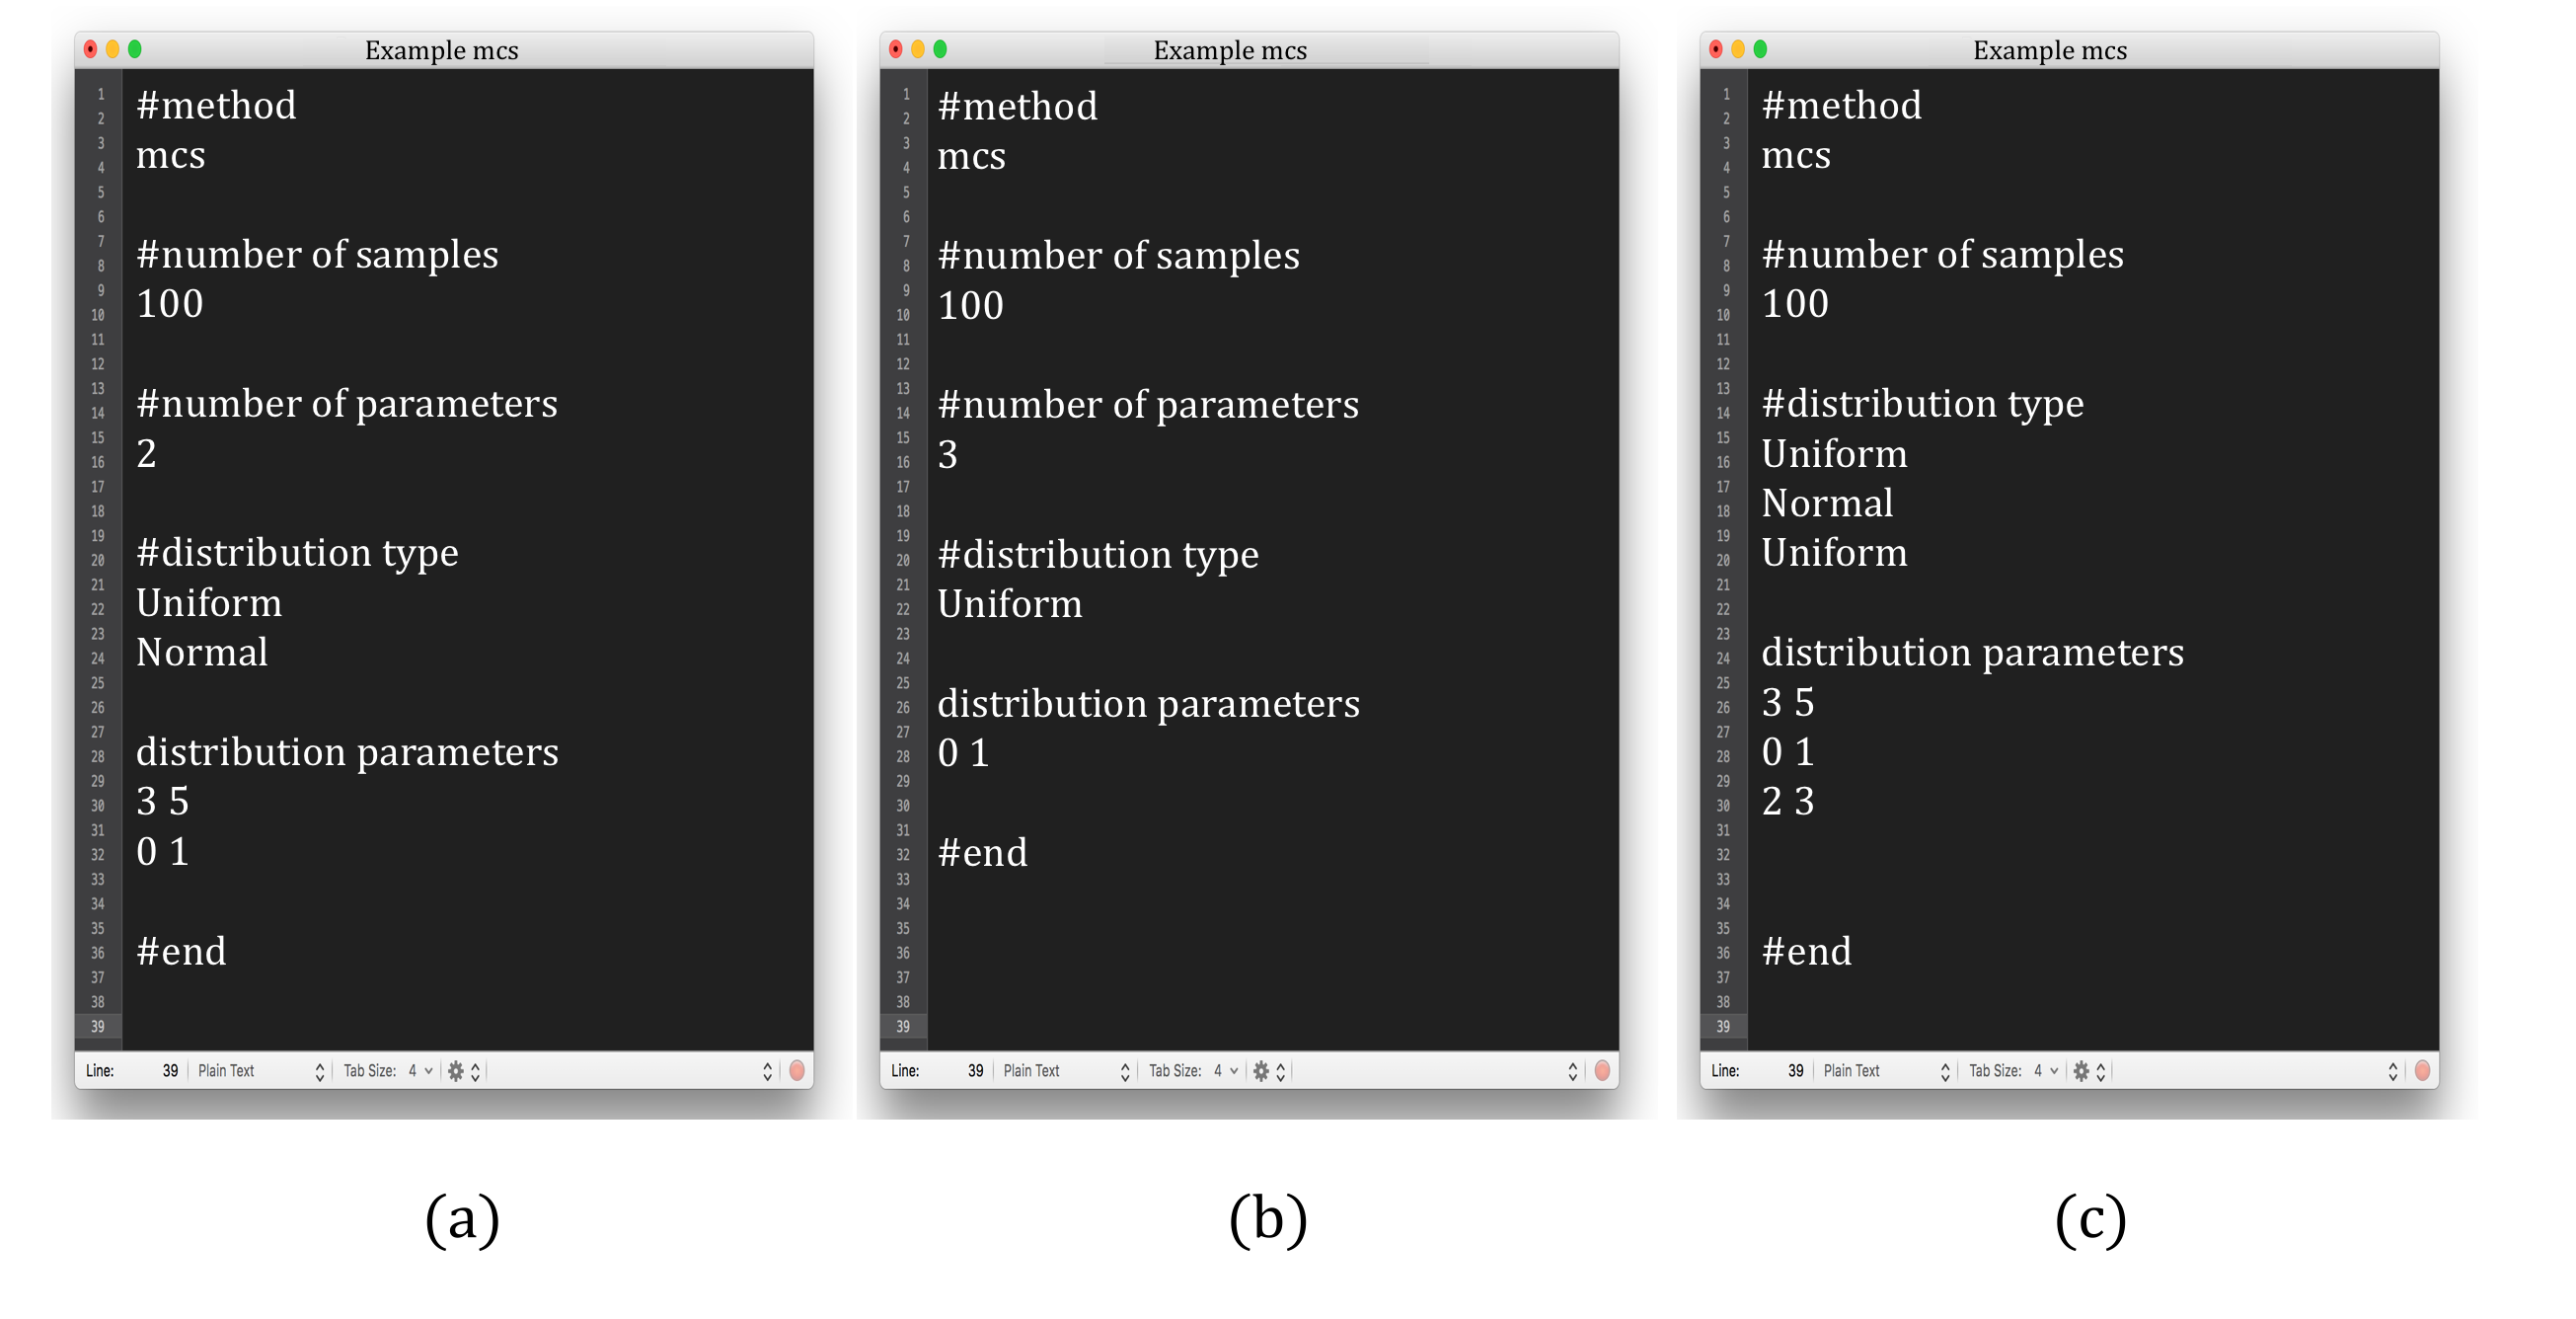
\includegraphics[scale=0.3]{template_mcs}}
	\caption{}
	\label{template_mcs}
\end{figure}



\subsection{Template Input File}

The functionality of the {\color{red} name2*.sh} bash shell script file is to convert the text-based output file of \texttt{UQpy}   ({\color{magenta} UQpy\_run\_i.txt}) that contains the realization {\color{magenta} i}  of the parameter vector into appropriate input  for the analysis code.  The user is responsible for creating the appropriate bash script for performing this action. For example, if the software code reads a text-based  file called {\color{magenta} modelInput\_i.txt} then a possible {\color{red} name2*.sh} script would be the one depicted in Fig.\ref{template_input};  it is used for renaming {\color{magenta} UQpy\_run\_i.txt } to {\color{magenta} modelInput\_i.txt}.


\begin{figure}[!ht]
	\centering	{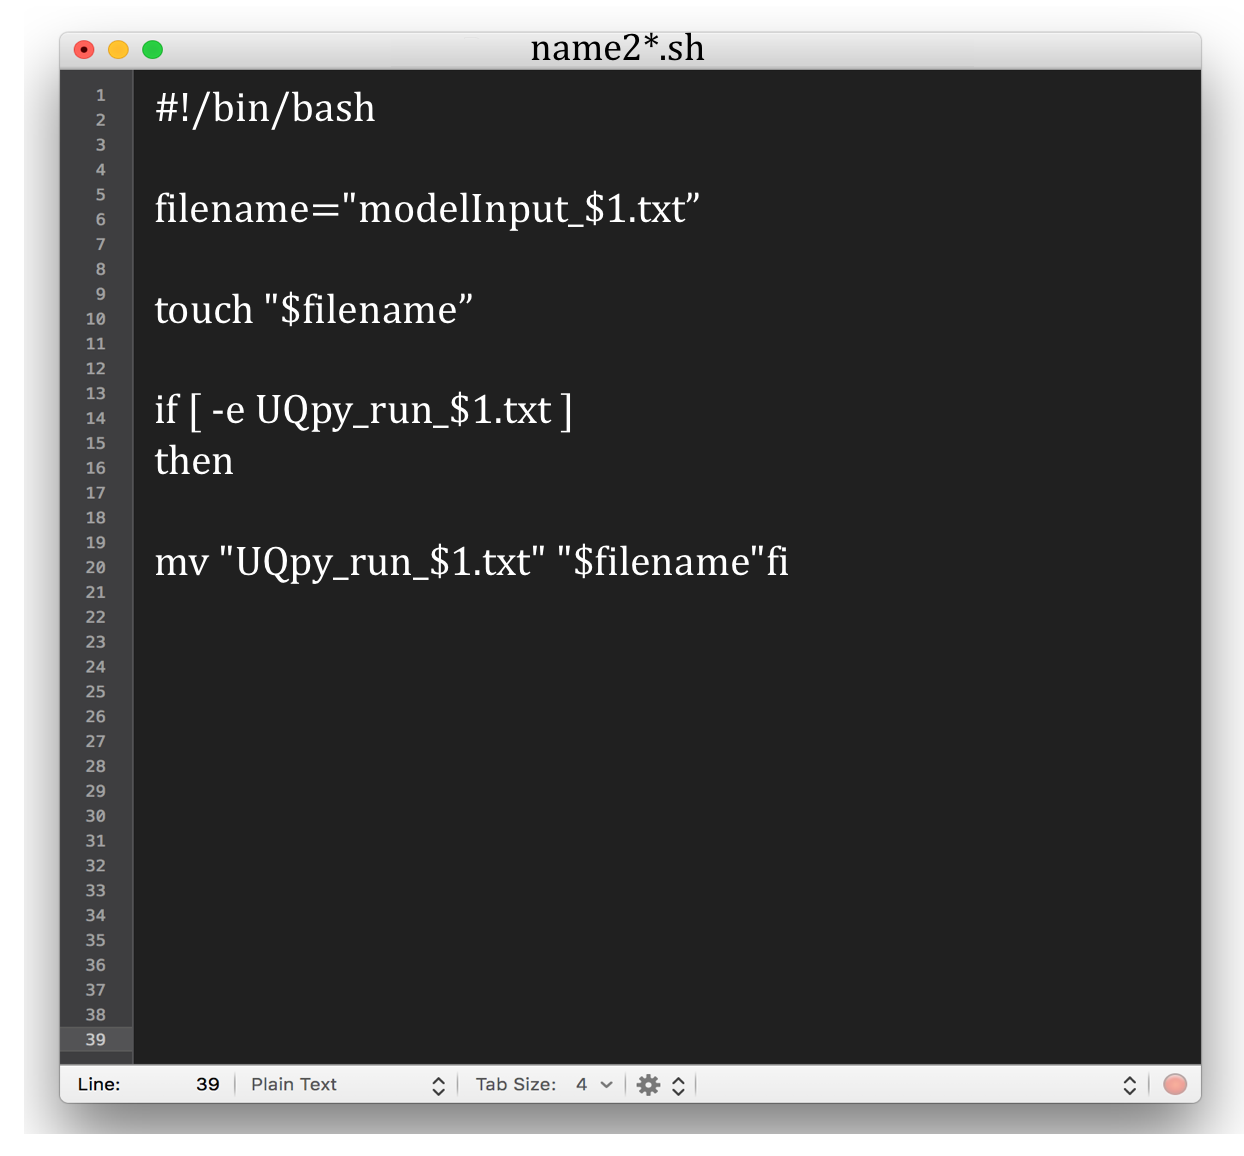
\includegraphics[scale=0.40]{template_input}}
	\caption{}
	\label{template_input}
\end{figure}



\subsection{Template Model File}

In order for \texttt{UQpy}  to execute the software code a bash script ({\color{red} name1*.sh} ) is necessary.  


\begin{figure}[!ht]
	\centering	{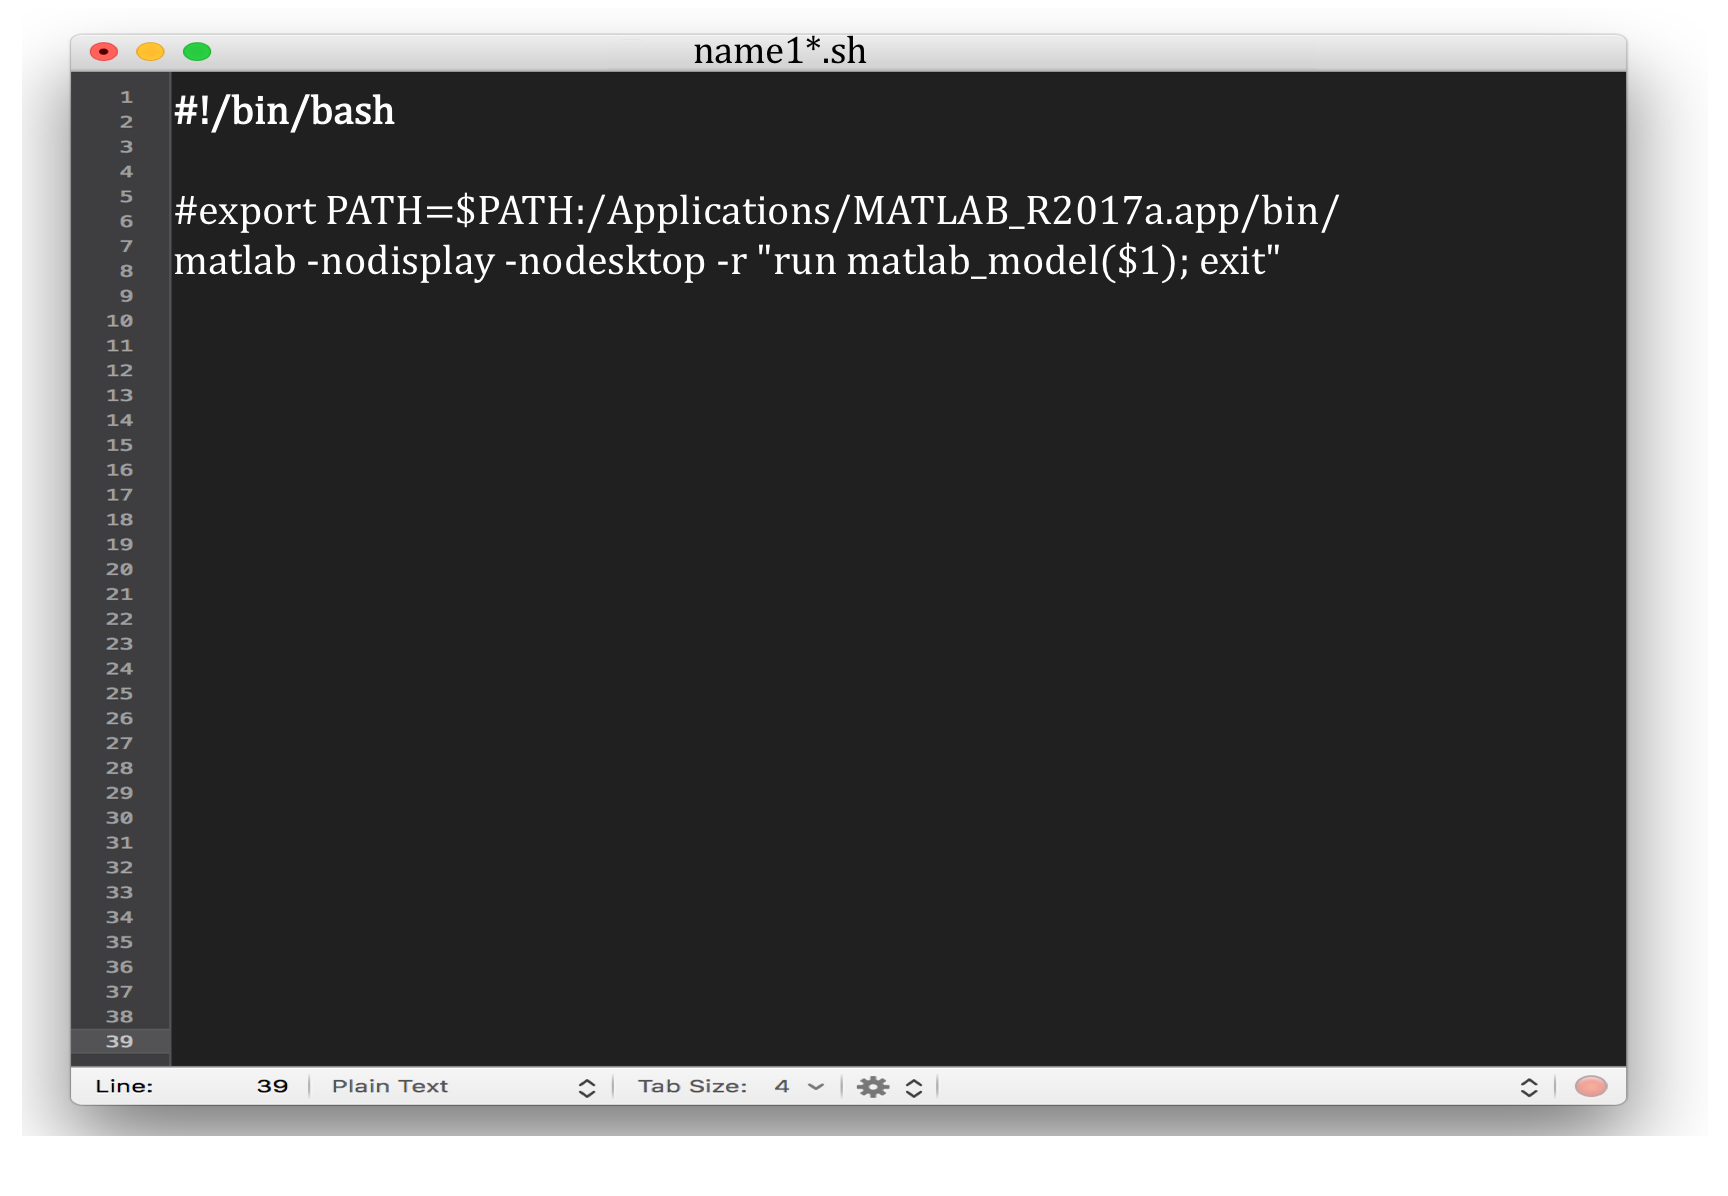
\includegraphics[scale=0.40]{template_model}}
	\caption{}
	\label{template_model}
\end{figure}



\subsection{Template Output File}

The functionality of the {\color{red} name3*.sh} bash shell script file is to convert the output of the code analysis (which can be at any format) into a text file file under the name {\color{magenta} UQpy\_eval\_i.txt"}, where {\color{magenta} i} refers to the number of simulation,  ready to be processed by \texttt{UQpy}. This step is required for running adaptive UQ methods as well as for post-processing of the result but in any case it is mandatory to provide such file. For example, if the software code generates a text-based  file called {\color{magenta} solution\_i.txt} then a possible {\color{red} name3*.sh} script would be the one depicted in Fig.\ref{template_output};  it is used for renaming {\color{magenta} solution\_i.txt} to {\color{magenta} UQpy\_eval\_i.txt"}.


\begin{figure}[!ht]
	\centering	{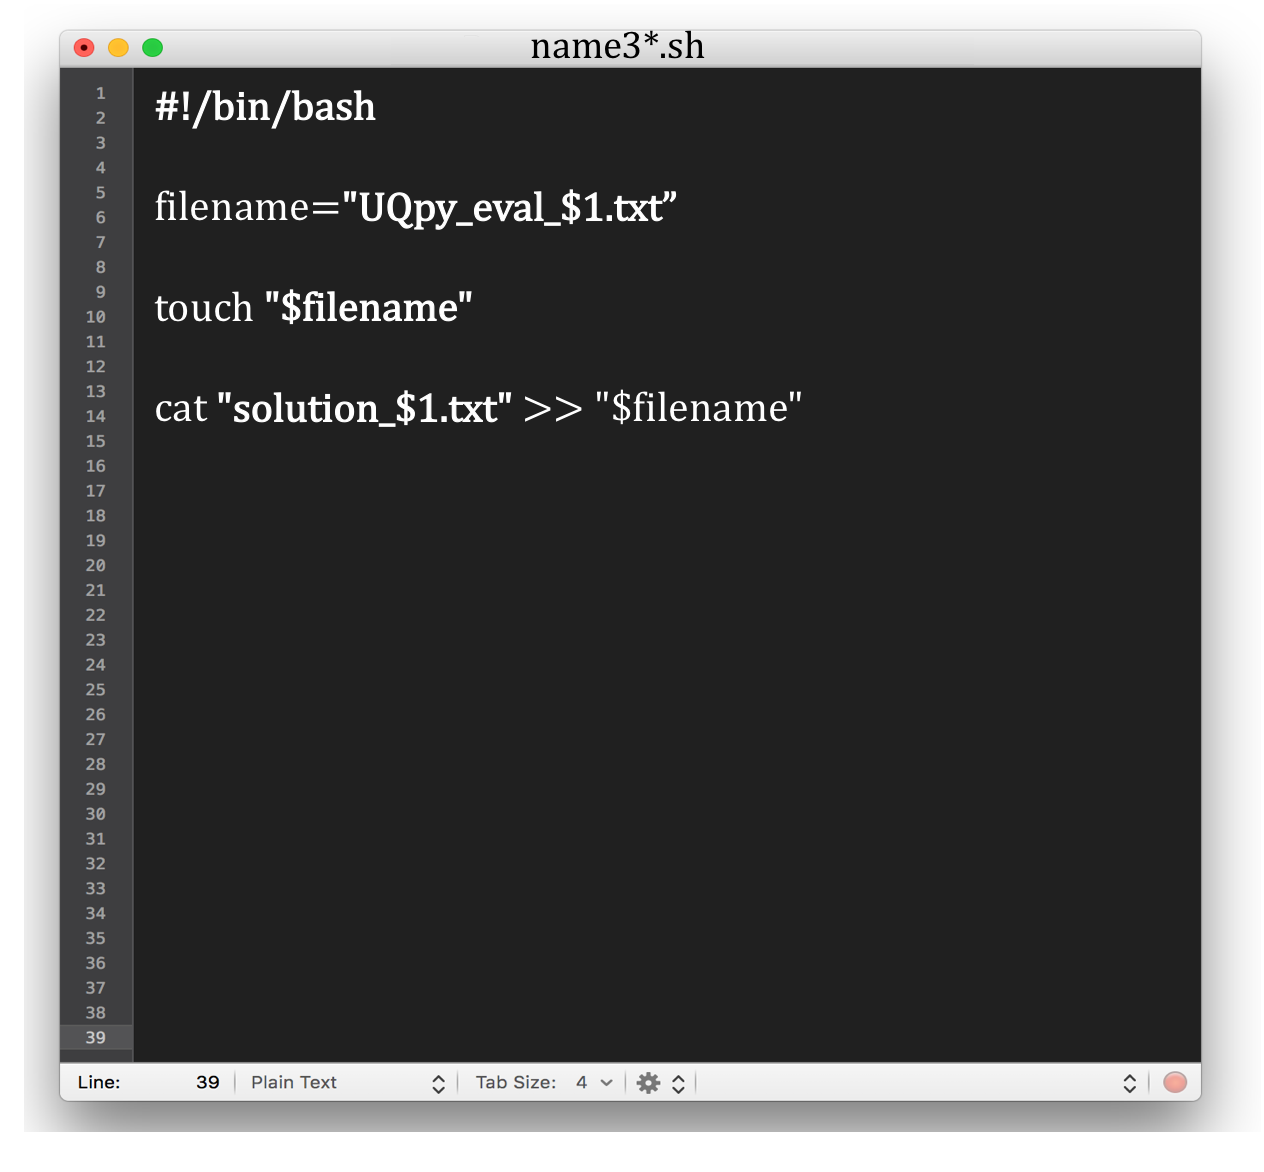
\includegraphics[scale=0.40]{template_output}}
	\caption{}
	\label{template_output}
\end{figure}

\subfile{Modules}


\section*{References}

\end{document}

%%
%% End of file `elsarticle-template-1-num.tex'.